\section{Component View}


This section details the internal modules used in each component seen previously.
in particular, we focus about the main subcomponents of the business logic layer, as described in the previous chapter concerning the architecture overview. 
this because the main functionalities  of our software are almost all exploited at this level, whereas the other layer's components are mainly
designed in order to guarantee non functional features such as scalability or security. 

At component level, the software can be divided betweeen \emph{front-end components} and \emph{back-end components}; as a five-layers architecture, the \emph{Travlendar+} frontend is mainly represented by the client layer, which, as described in the \emph{Requirement analysis and specification document}, will be implemented as a mobile application and as web application, usable via browser.
\subsection{Front-end system}
In this subsection we mainly focus on the analysis of a possible generic client application, which can be implemented as a native application but also as a browser-oriented frontend.
Nowadays it is relatively simple to develop javascript based applications which uses web-oriented technologies without having to deal with common web browsers. this is the reason why is
natural to describe the two client interfaces using a single component diagram: the overall structure is mainly similar, and the main differences are implementation related and thus not
discussed in this document.
\begin{figure}[H]
    \centering
    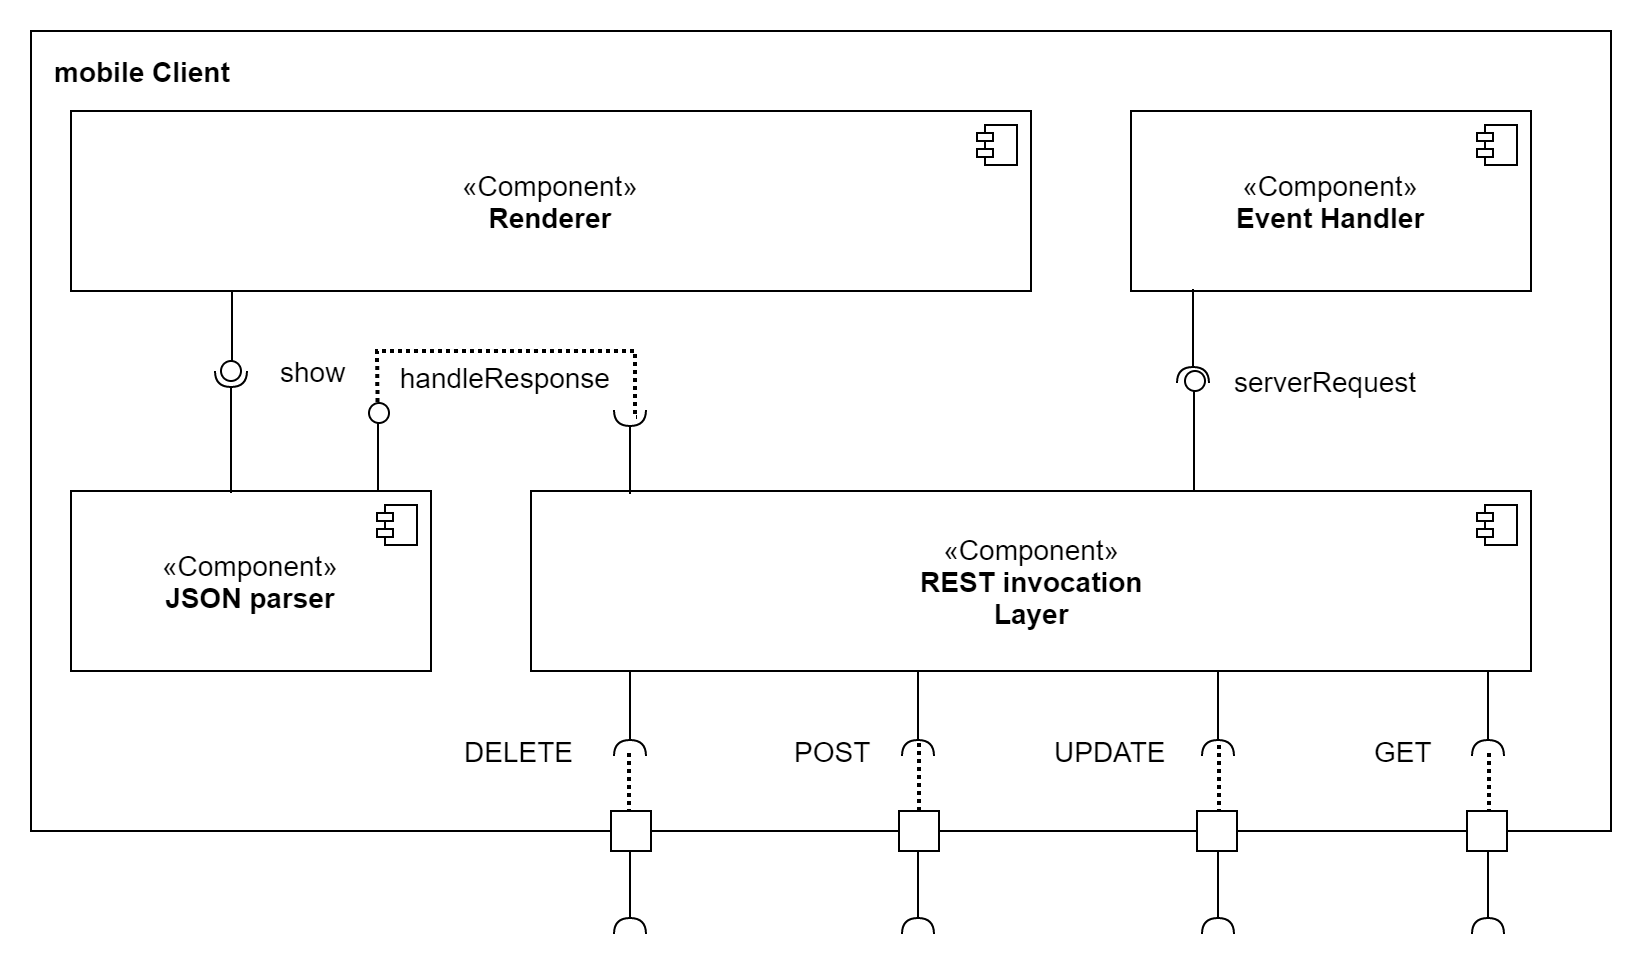
\includegraphics[scale=0.2]{Pictures/ComponentDiagram/client_component.png}
    \caption{UML component diagram about front-end components}
    \label{component:client}
\end{figure}

As seen in Figure \ref{component:client}, the main components are:
\begin{itemize}
    \item \textbf{the Renderer}: this component is meant to show datas from the back end and display the interface from whom the user interacts whith the application.
                                 in particular, the renderer is designed to be observed by other components, as in a traditional \emph{observable - observer pattern}:
                                 this choice has been made in order to make the renderer as much indipendent as possible with respect to the overrall application, and
                                 vice versa, thus permitting to  
    \item \textbf{the JSON parser}
    \item \textbf{the event handler}
    \item \textbf{the REST invocation layer}:
\end{itemize}


\subsection{Back-end system}
\newpage
\begin{figure}[H]
    \centering
    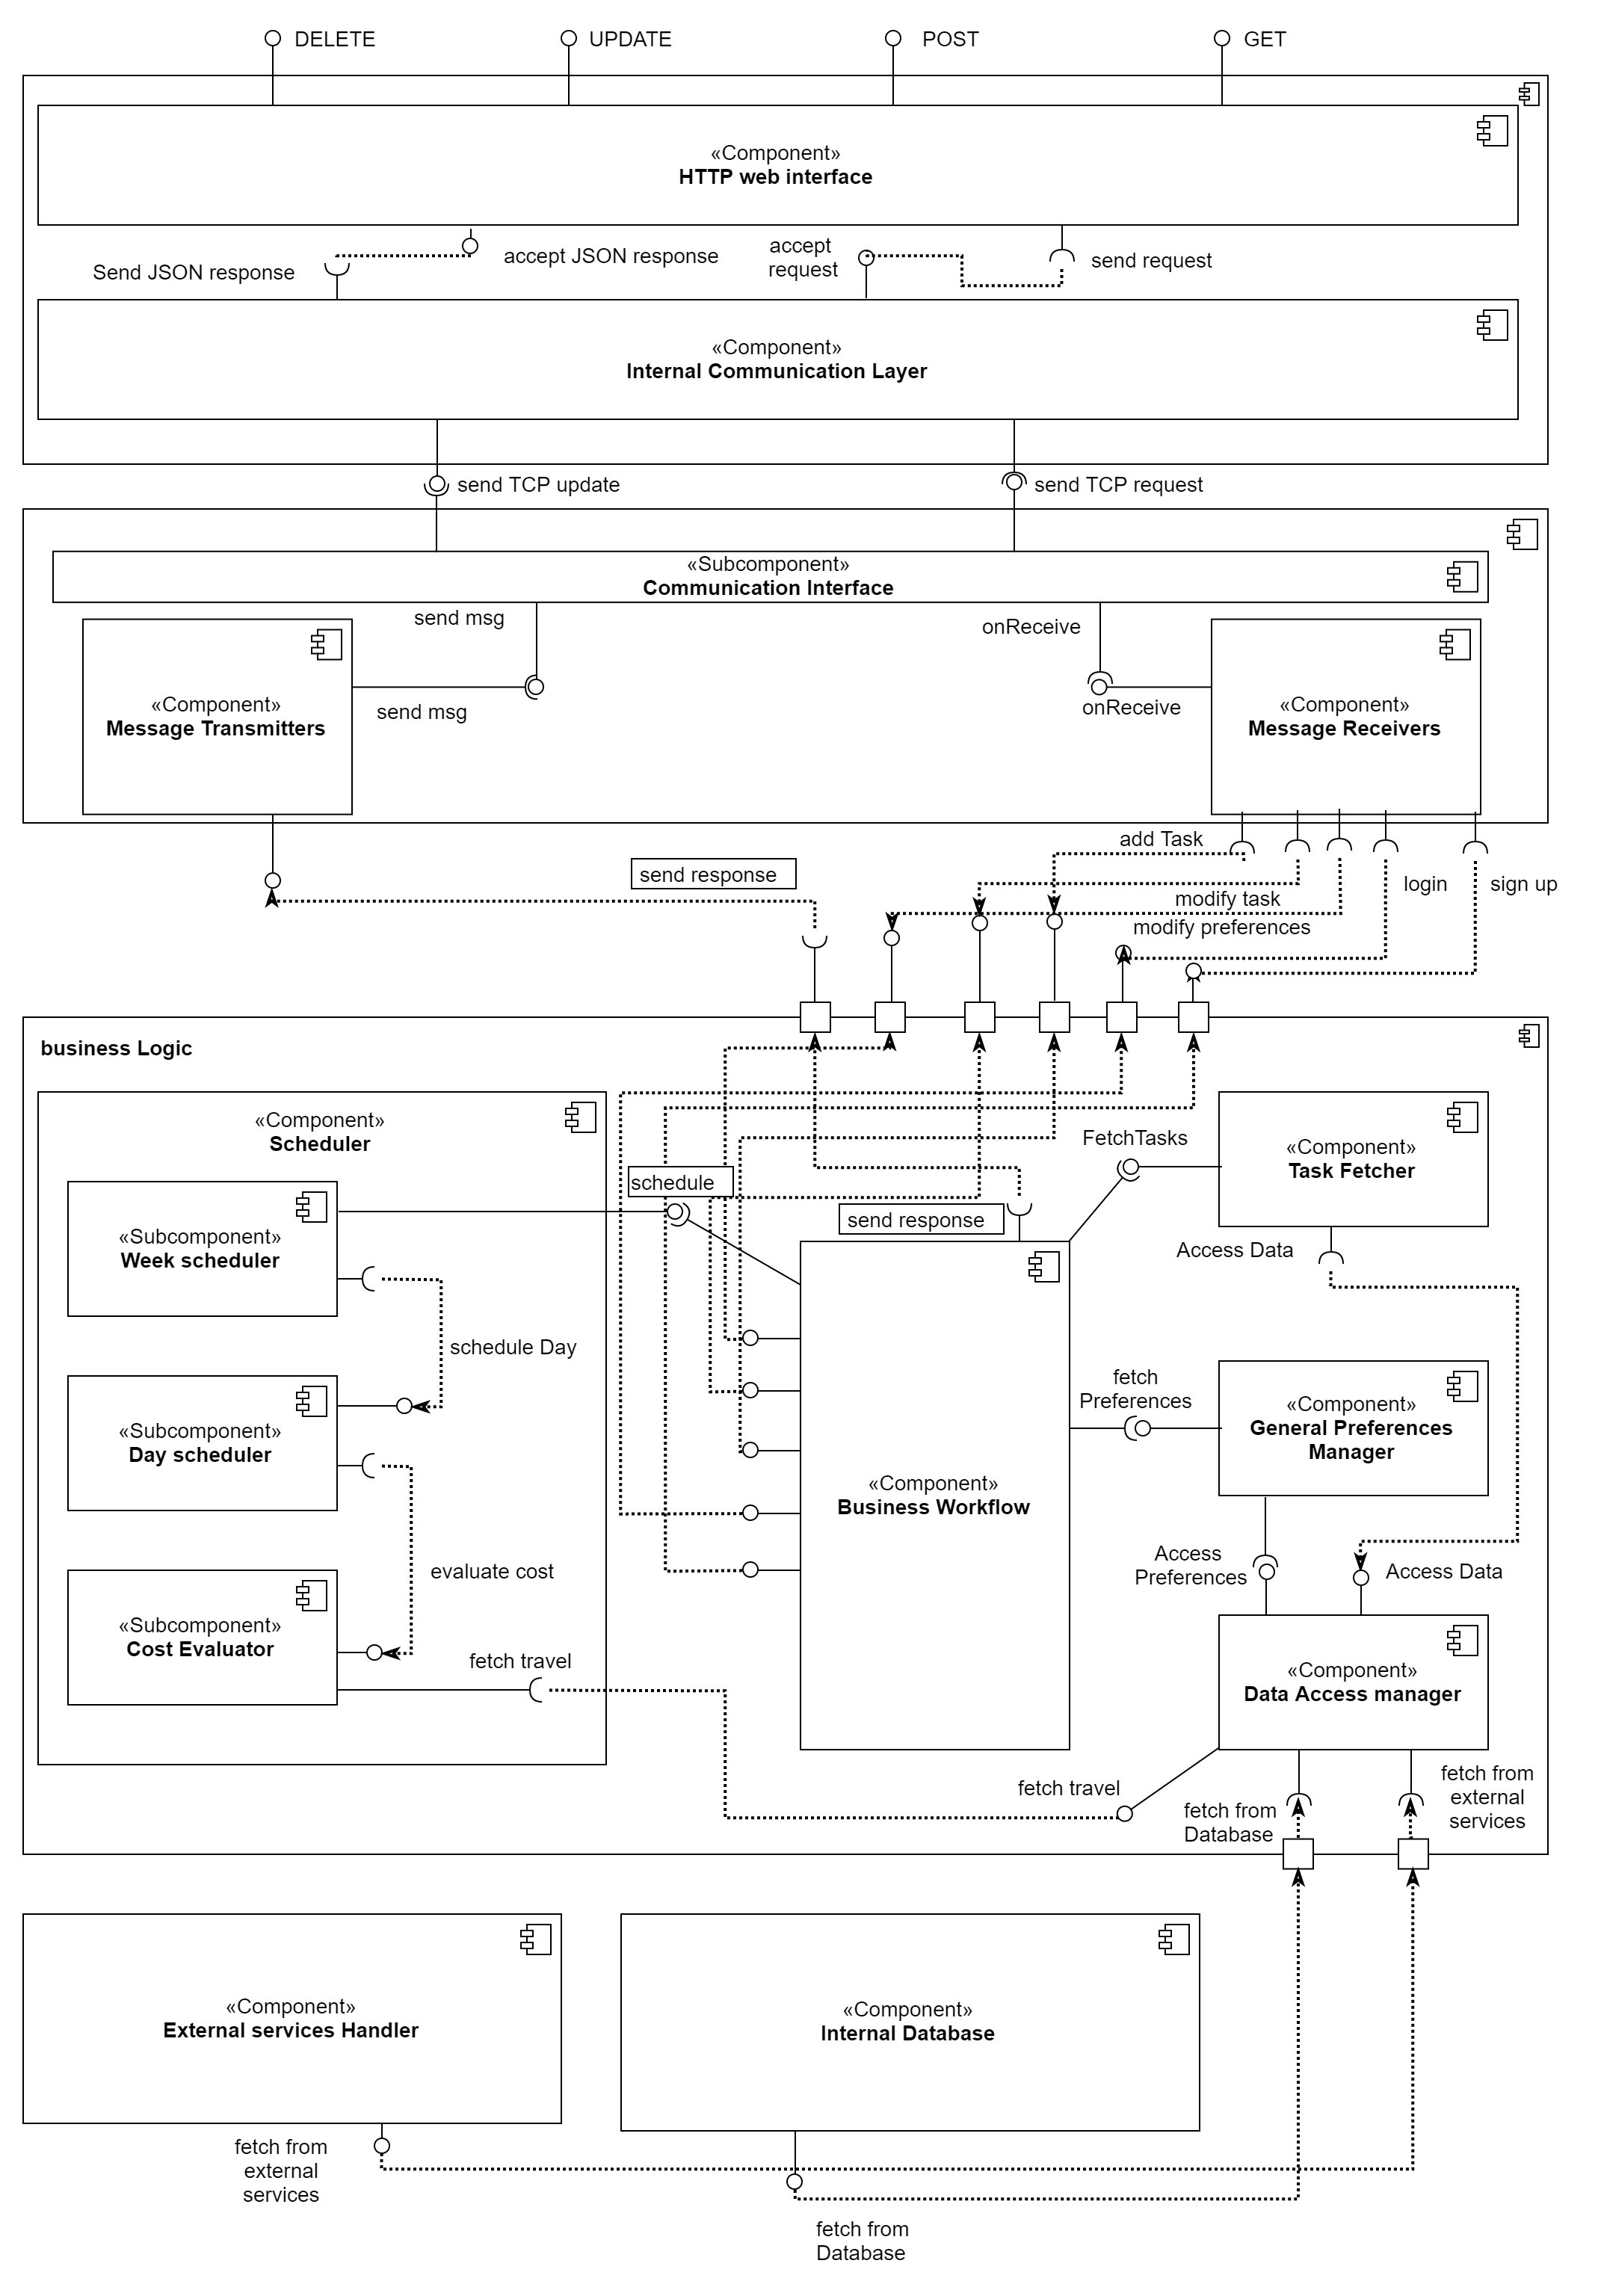
\includegraphics[scale=0.2]{Pictures/ComponentDiagram/componentDiagram.png}
    \caption{UML component diagram about back-end components}
\end{figure}

